\section{Beyond the Standard Model extensions of \ssww}\label{ssww13tev:extensions}
Many so-called \emph{Beyond the Standard Model} (BSM) theories exist that incorporate new physics with what has been experimentally observed.
BSM theories often manifest as deviations from the expected SM cross sections, either due to additional decay possibilities affecting branching ratios or modifications of the coupings themselves.
One of the most well-known avenues for BSM involving new particles is supersymmetry~\cite{1997.susy-primer}; however, two popular BSM extensions relevant to the \ssww process involve a doubly-charged Higgs particle ($H^{\pm\pm}$) and anomalous triple and quartic gauge couplings (aTGC and aQGC, respectively)\footnote{The aQGC's are the focus in this section since the $WWWW$ QGC vertex is accessible through \sswwnojj scattering, as well as the fact that aTGC's have been studied in far greater detail due to being accessibile through a larger number of processes.}.
These two BSM theories will be touched on in the context of \ssww analyses at the LHC.

\subsection{Doubly charged Higgs bosons}\label{ssww13tev:hpp}
Same-sign \sswwnojj scattering in the SM does not contain the $s$-channel diagram shown in Figure~\ref{fig:ssww13tev_diagrams_vbs}, as there is no SM resonance with $\pm 2$ electric charge; however, there are BSM theories that involve expanded Higgs sectors that do include such a particle.

One popular model is the Georgi-Machacek (GM) Higgs-triplet model~\cite{1985.doubly-charged-higgs}. 
The GM model proposes a Higgs triplet field $\chi$ in addition to the usual Higgs doublet $\phi$.
After symmetry breaking, each field obtains its own VEV, $v_\chi$ and $v_\phi$, and the SM VEV is made up of a combination of the two:
\begin{equation}
  v_{\textrm{SM}}^2 = v_\phi^2+8 v_\chi^2 \approx (246\gev)^2
\end{equation}
As a result, the $W^\pm$ and $Z$ boson masses, which are determined by $v_{\textrm{SM}}$ in the SM, receive contributions from both VEV's here.
It is important to note that even though this fixes the value of $v_\phi^2+8 v_\chi^2$, the ratio $v_\phi/v_\chi$ is not determined.
Thus, there is no required hierarchy $v_\chi \muchless v_\phi$, and the phenomenology of electroweak bosons can differ from the SM without conflicting with current experimental results~\cite{2013.triplet-higgs-lhc}.
Ultimately, the GM model predicts additional Higgs particles, including a doubly-charged $H^{\pm\pm}$.

The GM model has been tested experimentally by CMS at $\sqrt{s} = 8\textrm{\ and\ }13\tev$ for the process $H^{\pm\pm}\rightarrow W^{\pm}W^{\pm}$~\cite{2015.ssww-8tev-cms, 2017.ssww-13tev-cms}.
The coupling depends on the mass of the $H^{\pm\pm}$ as well as $s_H$, where $s_H^2$ is the fraction of the $W$ boson mass that is generated by $v_\chi$.
The resulting 95\% confidence level (CL) limits on the VBS cross section are shown in Figure~\ref{fig:cms-hpp-limits}.
Values of $s_H$ greater than $0.18$ and $0.44$ are excluded for $m_{H^{\pm\pm}} = 200\gev$ and $1\tev$, respectively.

\begin{figure}[htbp]
  \centering
  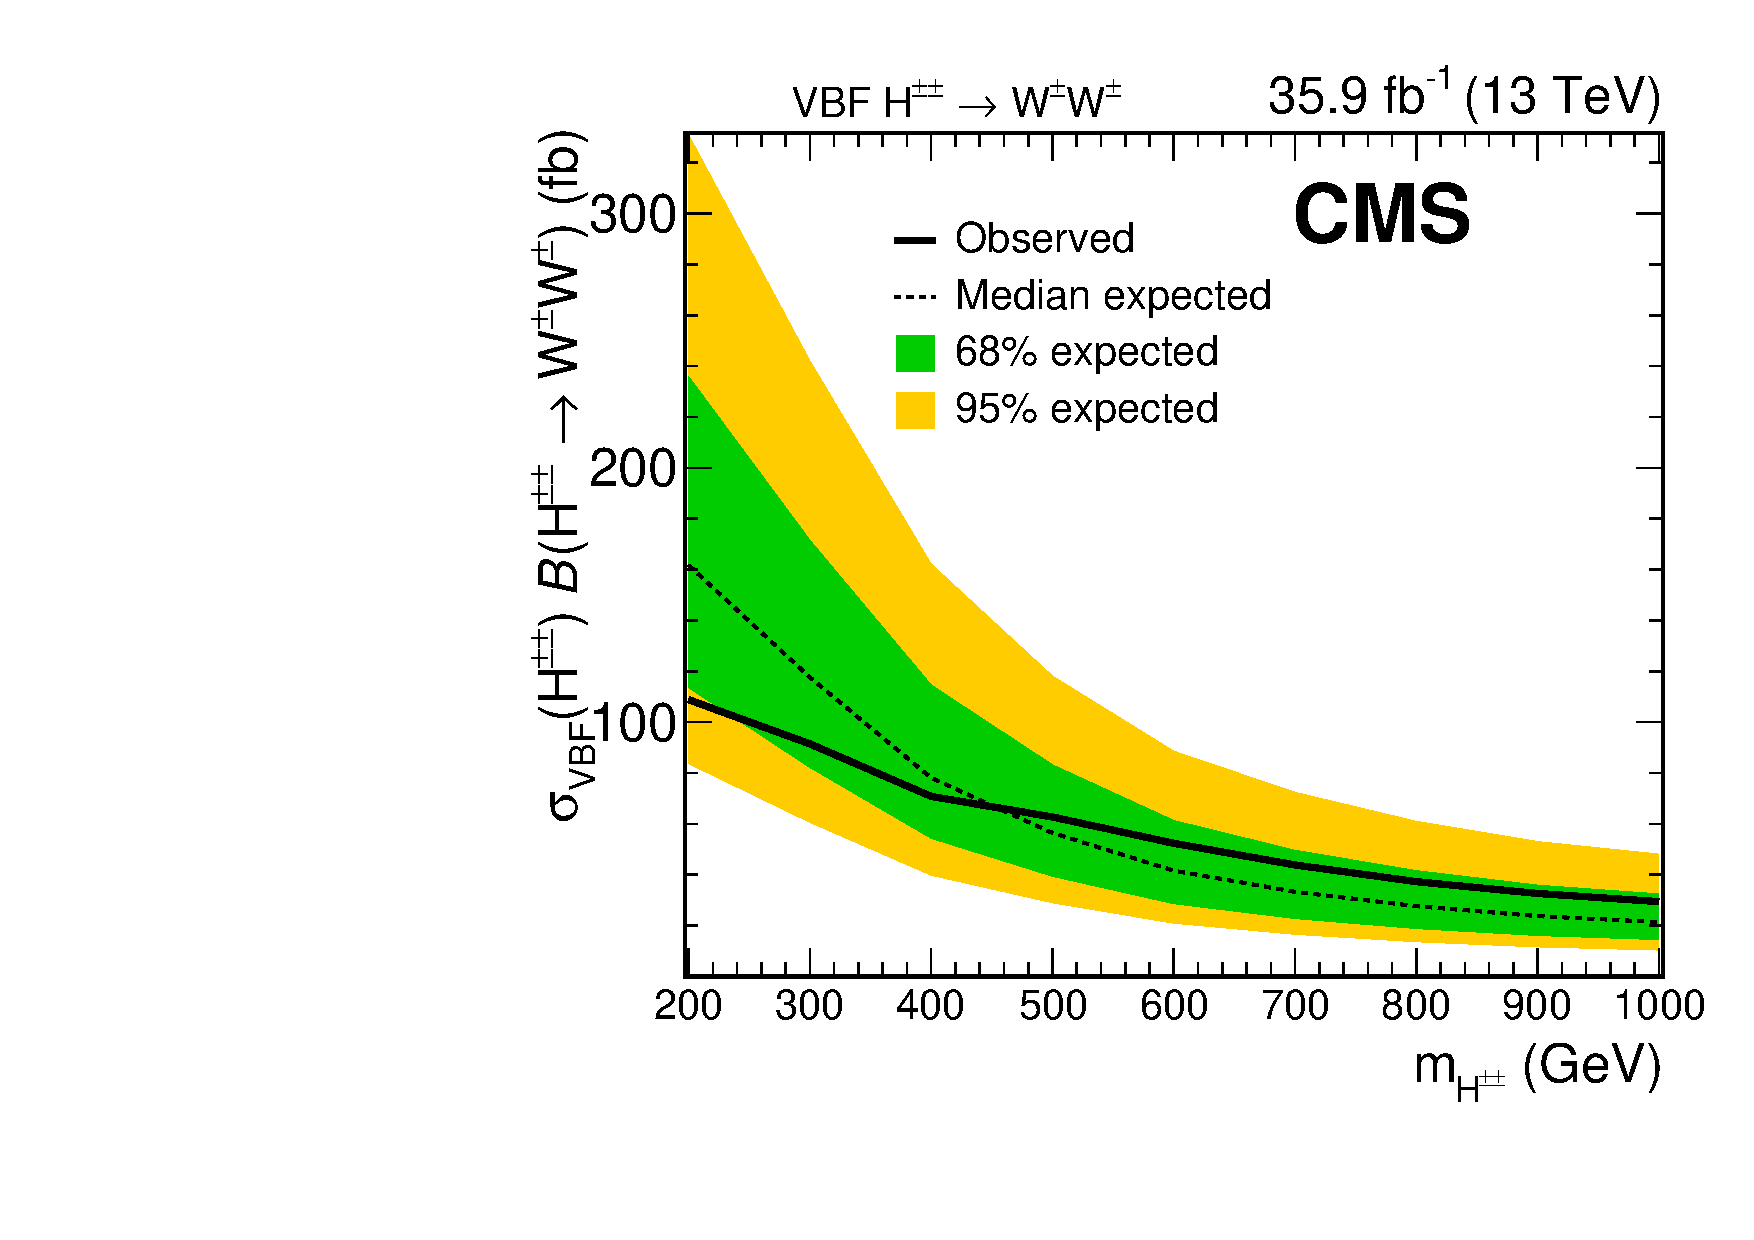
\includegraphics[width=.6\textwidth]{figs/ssww_13tev/extensions/cms-hpp}
  \caption[CMS observed and expected upper limits for the $H^{\pm\pm}\rightarrow W^{\pm}W^{\pm}$ cross section at 95\% CL at \com{13} as a function of $H^{\pm\pm}$ mass.  The region aboved the observed limit is excluded by the measurement.]{CMS observed and expected upper limits for the $H^{\pm\pm}\rightarrow W^{\pm}W^{\pm}$ cross section at 95\% CL at \com{13} as a function of $H^{\pm\pm}$ mass.  The region aboved the observed limit is excluded by the measurement. Plot taken from~\cite{2017.ssww-13tev-cms}.}
  \label{fig:cms-hpp-limits}
\end{figure}

A second model accounts for neutrino masses via a \emph{type II seesaw} mechanism, which involves extending the SM Higgs sector by a complex triplet of scalar fields with hypercharge $Y=2$~\cite{1980.neutrino-mass-higgs}.
This results in a similar situation as the GM model, with two VEV's $v_d$ and $v_t$ corresponding to the doublet and triplet fields, respectively, and multiple Higgs bosons, including a doubly-charged $H^{\pm\pm}$.
In this model, the relative sizes of the two VEV's is important for the context of the same-sign \sswwnojj process.
The observed neutrino masses are proportional to the size of $v_t$, which motivates a small value of the triplet VEV.
However, the $H^{\pm\pm}$ coupling to $W^\pm$ is also proportional to $v_t$, and for scenarios where $v_t \muchless v_d$, the $H^{\pm\pm}\rightarrow W^{\pm}W^{\pm}$ decay mode is suppressed~\cite{2008.type2-seesaw-lhc, 2011.higgs-type2-seesaw}.

This model has been studied by ATLAS at \com{13} involving pairs of $H^{\pm\pm}$ decaying to four $W^\pm$ bosons~\cite{2019.atlas-double-charged-higgs}.
The value of the triplet VEV is set to $v_t = 0.1\gev$, and the mass region $H^{\pm\pm} > 200\gev$ is considered.
No significant excess is seen above the SM predictions, and the 95\% CL limits on the $H^{\pm\pm}\rightarrow W^{\pm}W^{\pm}$ cross section are reproduced in Figure~\ref{fig:atlas-hpp-limits}.

\begin{figure}[htbp]
  \centering
  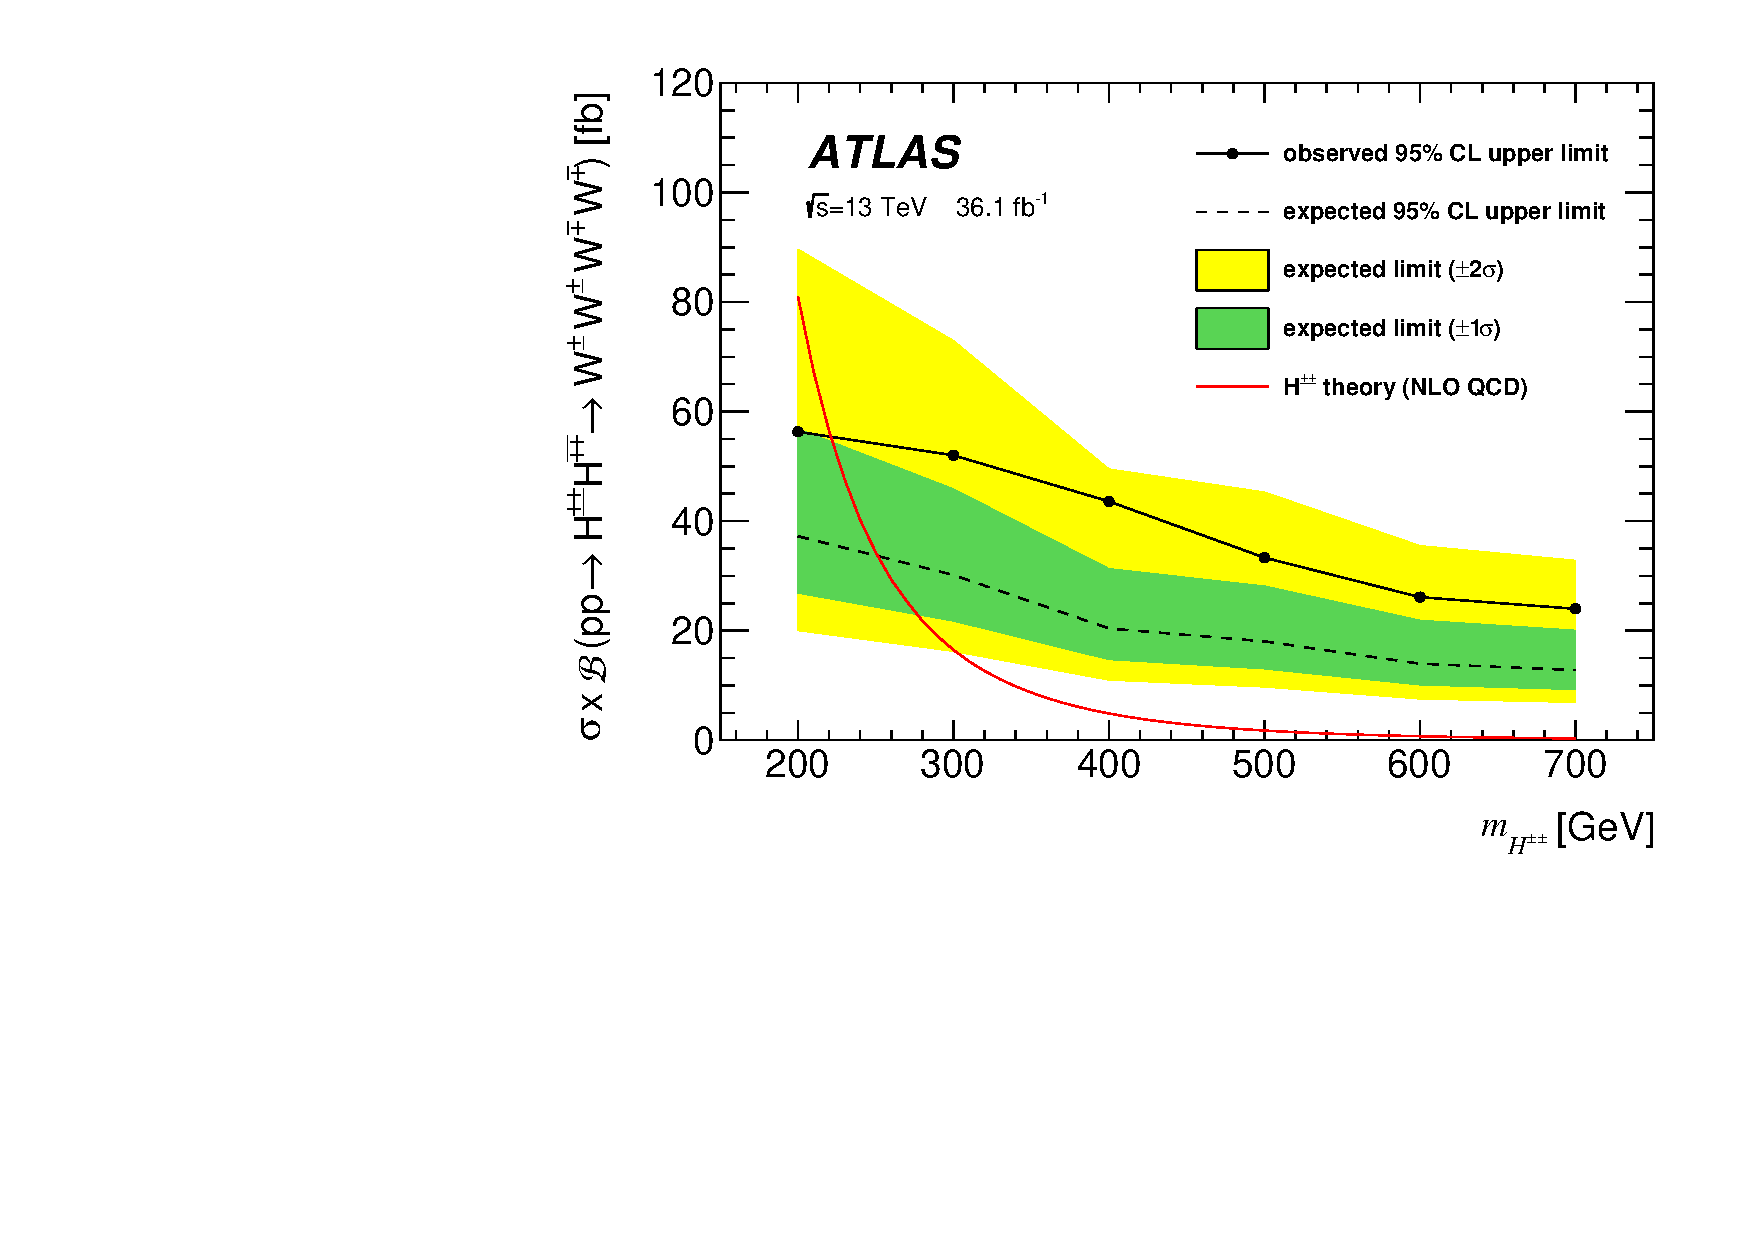
\includegraphics[width=.6\textwidth]{figs/ssww_13tev/extensions/atlas-hpp}
  \caption[ATLAS observed and expected upper limits for the $H^{\pm\pm}H^{\mp\mp}\rightarrow W^{\pm}W^{\pm}W^{\mp}W^{\mp}$ cross section at 95\% CL at \com{13} as a function of $H^{\pm\pm}$ mass.  The region aboved the observed limit is excluded by the measurement.]{ATLAS observed and expected upper limits for the $H^{\pm\pm}H^{\mp\mp}\rightarrow W^{\pm}W^{\pm}W^{\mp}W^{\mp}$ cross section at 95\% CL at \com{13} as a function of $H^{\pm\pm}$ mass.  The region aboved the observed limit is excluded by the measurement. Plot taken from~\cite{2019.atlas-double-charged-higgs}.}
  \label{fig:atlas-hpp-limits}
\end{figure}

\subsection{Anomalous quartic couplings}\label{ssww13tef:aqgc}
In the event that new physics exists at an energy scale far above what is currently accessible at the LHC, it cannot be directly observed by the experiment; however, its effects can still appear in the interactions between known particles.
In this case, the SM is simply the low-energy behavior of a larger \emph{effective field theory} (EFT), which contains additional, higher-dimensional operators that obey the existing SM symmetries:
\begin{equation}
  \mathcal{L}_{EFT} = \mathcal{L}_{SM}+\sum\limits_{d > 4}\sum\limits_i \frac{\tilde{c}_{i}}{\Lambda^{d-4}}\mathcal{O}_{i}
  \label{eq:eft_lagrangian}
\end{equation}
where $\mathcal{O}_i$ are operators of dimension $d$ with coefficients $\tilde{c}_i$, and $\Lambda$ is the energy scale of the new physics.
Here it can be clearly seen that as the energy scale $\Lambda\rightarrow\infty$, the SM behavior dominates.
In the region where $E\muchless\Lambda$, operators with high dimensionality contribute less to the total Lagrangian, and the summation may be truncated above a chosen value of $d$, at which point $\mathcal{L}_{EFT}$ becomes predictive and can parametrize any heavy new physics~\cite{2013.aqgc-mc}.

%EFT models are appealing due to the fact that they use the existing fields and symmetries of the SM and are consistent with existing SM results (since there is no current evidence for new physics) in the $\Lambda\rightarrow\infty$ limit.
%In this limit, these operators' contributions to observables can be estimated perturbatively in $(E/\Lambda)$~\cite{2017.multiboson-at-lhc}.
%The EFT can be written in terms of the SM Lagrangian plus contributions from operators $\mathcal{O}$ of dimension $\Delta$:

Only operators with even dimensionality are allowed in order to conserve baryon and lepton numbers.
The largest contributions to $\mathcal{L}_{EFT}$ therefore come from operators with $d=6$; however, any of these operators which modify the QGC's also modify the TGC's.
As a result, these operators are better constrained by existing analyses with greater sensitivity to TGC's.
Operators with $d=8$ are the lowest that modify exclusively the QGC's, of which there are 18, and nine of them modify the $WWWW$ QGC accessible through same-sign \sswwnojj scattering~\cite{2006.aqgc-at-lhc, 2013.aqgc-mc}:
\begin{equation}
  \begin{aligned}
    &\mathcal{O}_{S,0} = \big[(D_\mu\Phi)^\dagger D_\nu\Phi\big]\times\big[(D^\mu\Phi)^\dagger D^\nu\Phi\big]\\
    &\mathcal{O}_{S,1} = \big[(D_\mu\Phi)^\dagger D^\mu\Phi\big]\times\big[(D_\nu\Phi)^\dagger D^\nu\Phi\big]\\
    &\mathcal{O}_{M,0} = \textrm{Tr}\big[\hat{W}_{\mu\nu}\hat{W}^{\mu\nu}\big]\times\big[(D_\beta\Phi)^\dagger D^\beta\Phi\big]\\
    &\mathcal{O}_{M,1} = \textrm{Tr}\big[\hat{W}_{\mu\nu}\hat{W}^{\nu\beta}\big]\times\big[(D_\beta\Phi)^\dagger D^\mu\Phi\big]\\
    &\mathcal{O}_{M,6} = \big[(D_\mu\Phi)^\dagger\hat{W}_{\beta\nu}\hat{W}^{\beta\nu}D^\mu\Phi\big]\\
    &\mathcal{O}_{M,7} = \big[(D_\mu\Phi)^\dagger\hat{W}_{\beta\nu}\hat{W}^{\beta\mu}D^\nu\Phi\big]\\
    &\mathcal{O}_{T,0} = \textrm{Tr}\big[\hat{W}_{\mu\nu}\hat{W}^{\mu\nu}\big]\times\textrm{Tr}\big[\hat{W}_{\alpha\beta}\hat{W}^{\alpha\beta}\big]\\
    &\mathcal{O}_{T,1} = \textrm{Tr}\big[\hat{W}_{\alpha\nu}\hat{W}^{\mu\beta}\big]\times\textrm{Tr}\big[\hat{W}_{\mu\beta}\hat{W}^{\alpha\nu}\big]\\
    &\mathcal{O}_{T,2} = \textrm{Tr}\big[\hat{W}_{\alpha\mu}\hat{W}^{\mu\beta}\big]\times\textrm{Tr}\big[\hat{W}_{\beta\nu}\hat{W}^{\nu\alpha}\big]\\
  \end{aligned}
  \label{eq:aqgc_dim8}
\end{equation}
Each operator is paired with a coupling in the Lagrangian term: $\mathcal{L}_{S,0} = \frac{f_{S,0}}{\Lambda^4}\mathcal{O}_{S,0}$ and so on.
The SM prediction can be compared to simulations generated with chosen values for the anomalous coupling constants, as shown in Figure~\ref{fig:ssww13tev_aqgc}.

\begin{figure}
  \centering
  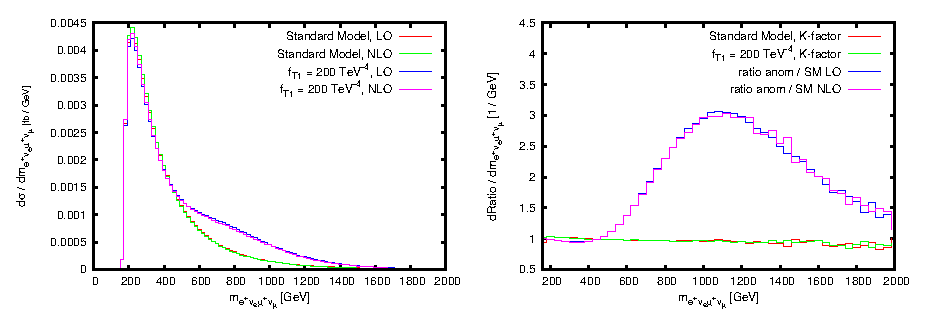
\includegraphics[width=.95\textwidth]{figs/ssww_13tev/extensions/aqgc}
  \caption[Invariant mass distributions of the $2l2\nu$ system in $pp\rightarrow e^{+}\nu_{e}\mu^{+}\nu_{\mu}jj$ events at LO and NLO with the \tt{VBFNLO} MC generator.  SM predictions are compared to those with the anomalous coupling $\frac{f_{T,1}}{\Lambda^4} = 200\tev^{-4}$.  The left plot shows the differential cross section for each prediction, and the right plot shows the $K$-factors for the SM and anomalous coupling predictions as well as the cross section ratio between the anomalous coupling and SM predictions at LO and NLO.]{Invariant mass distributions of the $2l2\nu$ system in $pp\rightarrow e^{+}\nu_{e}\mu^{+}\nu_{\mu}jj$ events at LO and NLO with the \tt{VBFNLO} MC generator.  SM predictions are compared to those with the anomalous coupling $\frac{f_{T,1}}{\Lambda^4} = 200\tev^{-4}$.  The left plot shows the differential cross section for each prediction, and the right plot shows the $K$-factors for the SM and anomalous coupling predictions as well as the cross section ratio between the anomalous coupling and SM predictions at LO and NLO.  Plots taken from~\cite{2013.aqgc-mc}.}
  \label{fig:ssww13tev_aqgc}
\end{figure}

Limits on the anomalous couplings generated by the $d=8$ operators of Equation~\ref{eq:aqgc_dim8} have been set by CMS in their \ssww analyses at $\sqrt{s} = 8\textrm{\ and\ }13\tev$~\cite{2015.ssww-8tev-cms, 2017.ssww-13tev-cms}.
ATLAS has also set limits at \com{8}~\cite{2014.ssww-8tev-atlas} using a different parameterization of the anomalous couplings outlined in~\cite{2013.aqgc-alpha}.
The limits set in CMS's $13\tev$ analysis are reproduced in Table~\ref{tab:aqgc_cms}.
The limits are obtained from fits to the $m_{ll}$ distributions in the signal and $WZ$ control regions, and 95\% confidence intervals are calculated by varying each operator individually.

\begin{table}[htbp]
  \centering
  \begin{tabular}{l c}
    Coupling & Observed limits $[\textrm{TeV}^{-4}]$ \\
    \hline\hline
    $f_{S,0}/\Lambda^4$ & $[-7.7, 7.7]$ \\
    $f_{S,1}/\Lambda^4$ & $[-21.6, 21.8]$ \\
    $f_{M,0}/\Lambda^4$ & $[-6.0, 5.9]$ \\
    $f_{M,1}/\Lambda^4$ & $[-8.7, 9.1]$ \\
    $f_{M,6}/\Lambda^4$ & $[-11.9, 11.8]$ \\
    $f_{M,7}/\Lambda^4$ & $[-13.3, 12.9]$ \\
    $f_{T,0}/\Lambda^4$ & $[-0.62, 0.65]$ \\
    $f_{T,1}/\Lambda^4$ & $[-0.28, 0.31]$ \\
    $f_{T,2}/\Lambda^4$ & $[-0.89, 1.02]$ \\
    \hline
  \end{tabular}
  \caption[Observed 95\% confidence limits set by CMS at \com{13} on the nine dimension-eight operators that modify the $WWWW$ QGC listed in Equation~\ref{eq:aqgc_dim8}.]{Observed 95\% confidence limits set by CMS at \com{13} on the nine dimension-eight operators that modify the $WWWW$ QGC listed in Equation~\ref{eq:aqgc_dim8}. Table taken from~\cite{2017.ssww-13tev-cms}.}
  \label{tab:aqgc_cms}
\end{table}
